\documentclass[11pt]{standalone}

\usepackage{helvet}

\usepackage{ifthen}
\usepackage{tikz} 
\usetikzlibrary{shapes.misc}
\usetikzlibrary{arrows,arrows.meta}
\usetikzlibrary{calc,intersections, patterns, math}

\definecolor{pfeil}{RGB}{168,167,167}
\definecolor{petrol}{RGB}{0, 118, 136}
\definecolor{darkgoldenrod}{RGB}{184, 134, 11}
\colorlet{petrol-lighter}{petrol!40}
\colorlet{darkgoldenrod-lighter}{darkgoldenrod!40}

\begin{document}

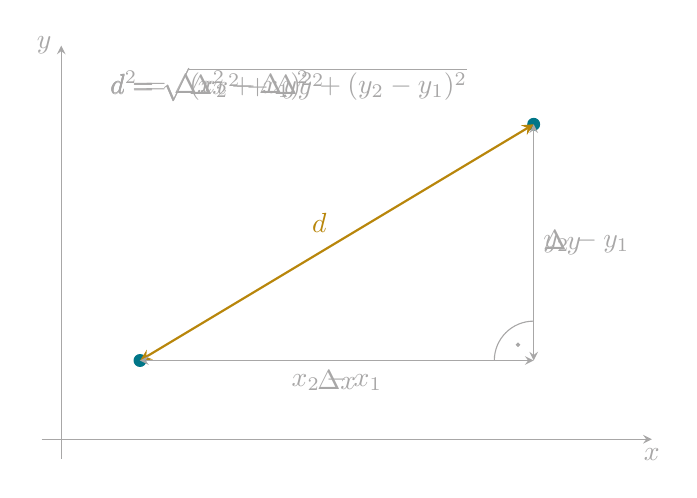
\begin{tikzpicture}[pfeil]

    % \draw[thick, fill=petrol!20, draw=petrol-lighter, rounded corners=2ex, opacity=0.5] (0,0) rectangle ++ (1.5,3.5);
    % \draw[thick, fill=darkgoldenrod!20, draw=darkgoldenrod-lighter, rounded corners=2ex, opacity=0.5] (5,0) rectangle ++ (1.5,3.5);

    \draw[-stealth] (-0.25,0) -- (7.5,0) node[below] {$x$};
    \draw[-stealth] (0,-0.25) -- (0,5)node[left]{$y$};

    \draw[petrol, fill] (1,1) circle (0.075);
    \draw[petrol, fill] (6,4) circle (0.075);
    \draw[thick, darkgoldenrod, stealth-stealth] (1,1) -- node[above left] {$d$} (6,4);


    \draw[stealth-stealth] (1,1) -- node[below]{$\Delta x$} (6,1);
    \path (1,1) -- node[below]{$x_2-x_1$} (6,1);
    \draw[stealth-stealth] (6,1) -- node[right]{$\Delta y$}  (6,4);
    \path (6,1) -- node[right]{$y_2-y_1$}  (6,4);


    \draw (5.5,1) arc(180:90:0.5);
    \draw[fill] (5.8,1.2) circle (0.02);


    \node[right] at (0.5,4.5) {$d^2=\Delta x^2 + \Delta y^2$};
    \node[right] at (0.5,4.5) {$d=\sqrt{\Delta x^2 + \Delta y^2}$};
    \node[right] at (0.5,4.5) {$d=\sqrt{(x_2-x_1)^2 + (y_2-y_1)^2}$};




\end{tikzpicture}

\end{document}
